%Dokumentklasse
\documentclass[a4paper,12pt,listof=totoc, bibliography=totoc]{scrreprt}
\usepackage[left= 2.5cm,right = 2cm, bottom = 3 cm, top = 2cm]{geometry}
%\usepackage[onehalfspacing]{setspace}
% ============= Packages =============

% subsubsection wird im Inhaltverzeichnis angezeigt
\setcounter{tocdepth}{5}
\setcounter{secnumdepth}{5}

\usepackage{listings}
\usepackage{xcolor}

% Dokumentinformationen
\usepackage[
	pdftitle={},
	pdfsubject={},
	pdfauthor={},
	pdfkeywords={}
	pdftex=true, 
	colorlinks=true,
 	breaklinks=true,
	citecolor=black,
	linkcolor=black,	
	menucolor=black,	
	urlcolor=black
]{hyperref}


% ============= Packages =============
\usepackage[utf8]{inputenc}
\usepackage[english]{babel}
\usepackage[T1]{fontenc}
\usepackage{graphicx}
\usepackage{graphicx, subfigure}
\graphicspath{{img/}}
\usepackage{fancyhdr}
\usepackage{lmodern}
\usepackage{xcolor} % für verschiedene Farben
\usepackage{soul} % zum durchstreichen
\usepackage{transparent}
\usepackage{listings}
\usepackage[acronym, toc, nopostdot, nonumberlist]{glossaries}
\usepackage[automake]{glossaries-extra}
\usepackage[style=ieee]{biblatex}
\usepackage{todonotes}
\usepackage{tabularx}
\usepackage{multirow}
\usepackage{makecell}
\usepackage{colortbl}
\usepackage{svg}
\usepackage{booktabs}
\usepackage[normalem]{ulem}

%Serifenlose Schrift
\renewcommand{\familydefault}{\sfdefault}
%Serifenlose Kapitälchen
\usepackage{kpfonts}

% zusätzliche Schriftzeichen der American Mathematical Society
\usepackage{amsfonts}
\usepackage{amsmath}

% nicht einrücken nach Absatz
\setlength{\parindent}{0pt}


% ============= Kopf- und Fußzeile =============
\pagestyle{fancy}
%
\lhead{}
\chead{}
\rhead{\slshape \leftmark}
%%
\lfoot{}
\cfoot{\thepage}
\rfoot{}
%%
\renewcommand{\headrulewidth}{0.4pt}
\renewcommand{\footrulewidth}{0pt}

% ============= Package Einstellungen & Sonstiges ============= 

%Use bibliography
\bibliography{literature} 

%Use Glossaries
\makeglossaries
%\makenoidxglossaries

%Besondere Trennungen
\hyphenchar\font=\string"7F
\hyphenation{De-zi-mal-tren-nung St-rei-fen-licht-scan-nern Routing-Tabel-le Gnu-tel-la-Netz-werk}


%römische Aufzählungen mit \RM{Zahl}
\newcommand{\RM}[1]{\MakeUppercase{\romannumeral #1}}

% ===================== Page-numbering formatting ==========================
\makeatletter
\newcommand\frontmatter{%
    \cleardoublepage
  %\@mainmatterfalse
  \pagenumbering{roman}}

\newcommand\mainmatter{%
    \cleardoublepage
 % \@mainmattertrue
  \pagenumbering{arabic}}

\newcommand\backmatter{%
  \if@openright
    \cleardoublepage
  \else
    \clearpage
  \fi
 % \@mainmatterfalse
   }
\makeatother

% ============= Dokumentbeginn =============

\begin{document}

%----------------------------------------------------------------------%
%      File Inclusion
%----------------------------------------------------------------------%
    \begin{titlepage}
\begin{center}
\begin{tabular}{p{\textwidth}}


\begin{center}

\includegraphics[scale=0.3]{img/logo-en.jpg}
\end{center}

\\

\begin{center}
\large{Faculty Applied Computer Sciences \\ \vspace{0.2cm}
Bachelor Künstliche Intelligenz / Artificial Intelligence \\}
\end{center}

\\
\\

\begin{center}
\LARGE{}
\end{center}
\\
\\





\begin{center}
\Large{CLIP4PII}\\ \vspace{0.2cm}
\vspace{0.5cm}
\end{center}

\begin{center}
\large{AI Project (Group 2) - Summer Semester 2024}
% \\ 
% Master of Science
% \\
% an der Technischen Hochschule Deggendorf}
\end{center}

\\
\\

\end{tabular}
\end{center}


\vspace{1.5cm}

\makebox[3.4cm][l]{Name:} \makebox[5.0cm][l]{MatrikelNr.:} 
\newline
\makebox[3.4cm][l]{Name:} \makebox[5.0cm][l]{MatrikelNr.:} 
\newline 
\makebox[3.4cm][l]{Name:} \makebox[5.0cm][l]{MatrikelNr.:} 
\newline 
% \makebox[3.4cm][l]{Name:} \makebox[5.0cm][l]{MatrikelNr.:} \\
% \newline 

\vspace{1cm}

\makebox[10.0cm][l]{Lecturer:}\\
\makebox[3.4cm][l]{Robert Aufschläger}\\
% \makebox[3.4cm][l]{} \makebox[5cm][l]{} \makebox[10.0cm][l]{xy}\\
\vspace{1.0cm}

\makebox[3.4cm][l]{}\newline
Deggendorf, xx. Month 20xx
\makebox[3.4cm][l]{}

\end{titlepage}





\frontmatter
    %\input{002_NonDisclosureNote.tex}
    %\printglossary[type=\acronymtype, nonumberlist]
    %\printglossaries
    % ---------- add acronyms here ----------------
\newacronym{HE}{HE}{Homomorphic Encryption}
\newacronym{DHE}{DHE}{Distributed Homomorphic Encryption}
\newacronym{Noise}{Noise}{Ein Fehler, welcher nach jeder Operation hinzugefügt wird}  
\newacronym{Bootstrappen}{Bootstrappen}{Erneuerung des verschlüsselten Textes zur Minderung der Noise} 
\newacronym{Schema}{Schema}{Umsetzung einer homomorphen Verschlüsselung}  
\newacronym{FHE}{FHE}{Fully Homomorphic Encryption}  
\newacronym{PHE}{PHE}{Partial Homomorphic Encryption}  
\newacronym{SHE}{SHE}{Somewhat Homomorphic Encryption} 
\newacronym{RLWE}{RLWE}{Ring Learning with Errors}
\newacronym{Noise-Budget}{Noise-Budget}{Das Budget an Noise, das eine Fehlerfreie Entschlüsselung gewährt}
\newacronym{CKKS}{CKKS}{Cheon-Kim-Kim-Song Homomorphic Encryption for Arithmetic of Approximate Numbers (HEAAN)}

\newacronym{BFV}{BFV}{Brakerski-Fan-Vercauteren}
\newacronym{BGV}{BGV}{Brakerski-Gentry-Vaikuntanathan}
\newacronym{RSA}{RSA}{Rivest-Shamir-Adleman}

\newacronym{ki}{KI}{Künstliche Intelligenz}
\newacronym{nn}{NN}{Neural Network}
\newacronym{ml}{ML}{Machine Learning}







%\glsaddall
\printglossary[type=\acronymtype,title=Acronyms]
%\printnoidxglossary[type=\acronymtype,title=Acronyms]
    \tableofcontents
\mainmatter
    \chapter{Das ist ein Kapitel}
So wird ein neues Kapitel erstellt.
\section{Das ist eine Sektion}
Eine Sektion eines Kapitels
\subsection{Das ist eine Untersektion}
Untersektion einer Sektion
\subsubsection{Das ist eine unter Untersektion}
Die letzte Stufe, eine Untersektion einer Untersektion
\section*{Das ist eine Sektion die nicht in der Gliederung auftaucht}
Durch ein * am Ende wird sie nicht in die Gliederung aufgenommen


    \chapter{Bilder}
\section{Bild mit Caption drunter}

Auf dem Bild \ref{fig:featuremap} ist eine Feature Map zu sehen

\begin{figure}[h]
  \centering
  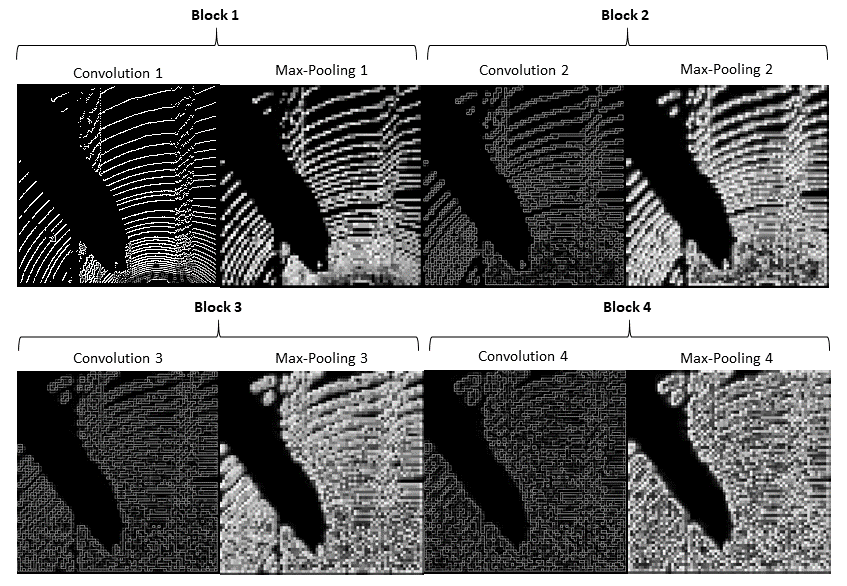
\includegraphics[width=\columnwidth]{img/feature_map.png}
  \caption{Illustration of the extraction of features from a 2D image consisting of LiDAR points, by means of a CNN.} \label{fig:featuremap}
\end{figure}


\section{Zwei Bilder nebeneinander}

Auf der Abbildung \ref{fig:fake_real_objects_examples} sind zwei Bilder zu sehen.

\begin{figure}
  \centering
  \subfigure[Real object with clear shadow]{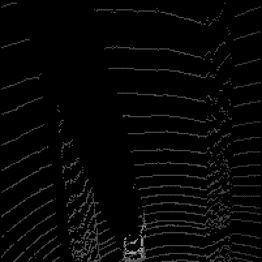
\includegraphics[width=0.45\textwidth]{img/shadowregion.png}}
  \subfigure[Spoofed Object without shadow]{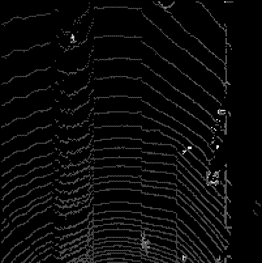
\includegraphics[width=0.45\textwidth]{img/spoofedregion.png}}
  \caption{Result of the 2D image generation, on the one hand with a true object (a) and on the other hand with a spoofed object (b).}
  \label{fig:fake_real_objects_examples} 
\end{figure}

\section{Drei Bilder nebeneinander}

Auf der Abbildung \ref{fig:dreibilder} sind drei Bilder zu sehen.

\begin{figure}[htbp]
    \subfigure[Ressourcen Allokation via Reinforcement Learning] {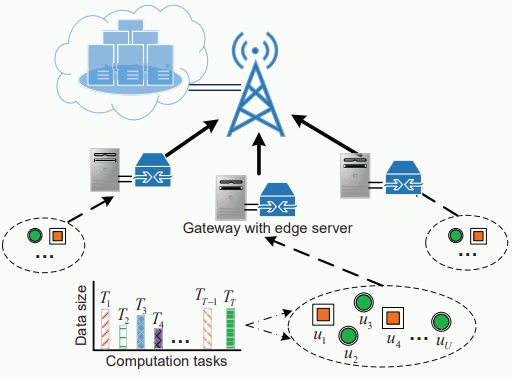
\includegraphics[width=0.33\textwidth]{jointtask07.PNG}}
    \subfigure[Erweitert mit verschiedenen Übertragungsmöglichkeiten] {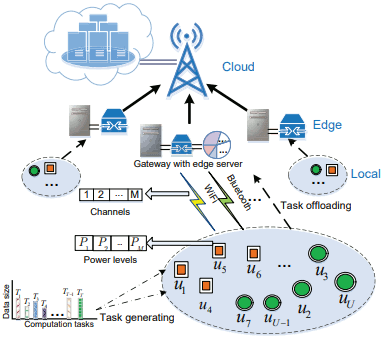
\includegraphics[width=0.33\textwidth]{jointtask05.PNG}} 
    \subfigure[Erweitert durch zentralisierten Clustering-Algorithmus] {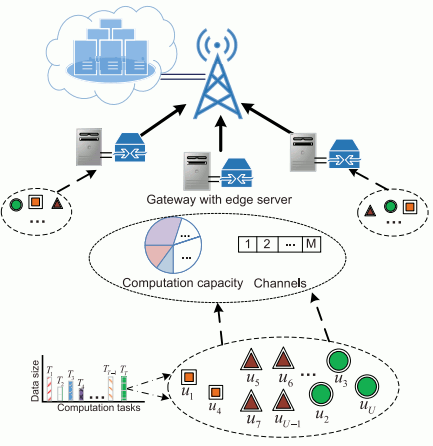
\includegraphics[width=0.33\textwidth]{jointtask08.PNG}}
\caption{Verschiedene Ressourcenallokierungsansätze} 
\label{fig:dreibilder}
\end{figure}


    \chapter{Mathe}
\section{Funktion Separat mit Referenz}

Hier ist die Sigmoidfunktion in \ref{eq:sigmoid} abgebildet. Sie wird in eine neue Zeile gesetzt.

\begin{equation} \label{eq:sigmoid}
    \large
    f(x) = \frac{1}{1+e^-\frac{net_j-\Theta}{T}}
\end{equation}

\section{Funktion in Fließtext eingearbeitet}

Hier ist die selbe Funktion noch einmal \(f(x) = \frac{1}{1+e^-\frac{net_j-\Theta}{T}}\) aber diesmal in den Text eingebettet

\section{Funktion Separat ohne Referenz}

Hier ist dieselbe Sigmoidfunktion \[f(x) = \frac{1}{1+e^-\frac{net_j-\Theta}{T}}\] Sie wird in eine neue Zeile gesetzt.
    \chapter{Formatierung}
\section{textbf}
\textbf{Fett Hervorgehoben:} text

\section{textit}
\textit{Kursiv:} text

\section{emph}
\emph{Kursiv:} Sieht aus wie Kursiv, wird aber auch hervorgehoben, wenn der ganze Text in Kursiv wäre. Beispiel: \textit{Der Befehl \emph{emph} sticht immer hervor!}

\section{Nicht alle Zeichen gehen}
Manche Zeichen sind für Latex reserviert dafür muss ein \(\backslash\) davor gesetzt werden. Beispiel \_ oder \%, viele andere mathematische Symbole haben spezielle Befehle, die verwendet werden müssen.
    \chapter{Tabellen}

\section{Beispiel 1}

Aus meiner Mastararbeit Beispiel \ref{tab:Software}

\begin{table}[ht]
  	\centering
  	\begin{tabular}{@{}*{4}{l}@{}}
  		\toprule
  		    \textbf{Software} & \textbf{Version} & \textbf{Software} & \textbf{Version}\\ 
  		\midrule
  		    Tensorflow & 2.4.0 &  Numpy & 1.19.4 \\
  		    Mininet & 2.3.0d6 & Pandas & 1.0.5 \\
  		    Ryu Controller & 4.34 & Dash & 1.13.4 \\
  		    Flask & 1.1.2 & Plotly & 5.1.0 \\
  		    Flask-Restful & 0.3.8 &  &  \\
  		\bottomrule
  	\end{tabular}
  	  	  \caption{Hauptsoftware, die verwendet wird}
  \label{tab:Software}
\end{table} 

\section{Beispiel 2}

IEE Paper Beispiel \ref{tab:cnn_sigmoid}

\begin{table}[h]
\caption{Architecture of the CNN SVM model}
\label{tab:cnn_sigmoid}
\centering
\begin{tabular}{c l c} 
\Xhline{1pt}
\textbf{Block} & \multicolumn{1}{c}{\textbf{Layer}}  & \textbf{Activation}  \\ 
\Xhline{1pt}
1     & \begin{tabular}[c]{@{}l@{}}Convolution (32 x 3 x 3)\\MaxPooling (2,2)\end{tabular}  & ReLU                                                  \\ 
\hline
2     & \begin{tabular}[c]{@{}l@{}}Convolution (64 x 3 x 3)\\MaxPooling (2,2)\end{tabular}  & ReLU                                                  \\ 
\hline
3     & \begin{tabular}[c]{@{}l@{}}Convolution (126 x 3 x 3)\\MaxPooling (2,2)\end{tabular} & ReLU                                                  \\ 
\hline
4     & \begin{tabular}[c]{@{}l@{}}Convolution (128 x 3 x 3)\\MaxPooling (2,2)\end{tabular} & ReLU                                                  \\ 
\hline
5     & \begin{tabular}[c]{@{}l@{}}Flattening\\Dense (512)\\Dense (1)\end{tabular}          & \begin{tabular}[c]{@{}c@{}}ReLU\\Sigmoid\end{tabular}  \\
\Xhline{1pt}
\end{tabular}
\end{table}


\section{Beispiel 3}

Eine farbige Tabelle \ref{tab:cnn_sigmoid_color}

\begin{table}[h]
\centering
\begin{tabular}{|c|l|c|} 
\hline
\rowcolor{yellow}
\textbf{Block} & \textbf{Layer}                                                                               & \textbf{Activation}                                            \\ 
\hline
1     & \begin{tabular}[c]{@{}l@{}}Convolution (32 x 3 x 3)\\MaxPooling (2,2)\end{tabular}  & ReLU                                                  \\ 
\hline
2     & \begin{tabular}[c]{@{}l@{}}Convolution (64 x 3 x 3)\\MaxPooling (2,2)\end{tabular}  & ReLU                                                  \\ 
\hline
3     & \begin{tabular}[c]{@{}l@{}}Convolution (126 x 3 x 3)\\MaxPooling (2,2)\end{tabular} & ReLU                                                  \\ 
\hline
4     & \begin{tabular}[c]{@{}l@{}}Convolution (128 x 3 x 3)\\MaxPooling (2,2)\end{tabular} & ReLU                                                  \\ 
\hline
5     & \begin{tabular}[c]{@{}l@{}}Flattening\\Dense (512)\\Dense (1)\end{tabular}          & \begin{tabular}[c]{@{}c@{}}ReLU\\Sigmoid\end{tabular}  \\
\hline
\end{tabular}
\caption{Architecture of the CNN SVM model}
\label{tab:cnn_sigmoid_color}
\end{table}
    \chapter{Bonus}

\section{Bash Umgebung}

\noindent Bash Befehl Beispiel:
\begin{lstlisting}[language=bash]
  $ df -h
  $ sudo umount /dev/sdb1
  $ dd if=/downloadpfad/imagename of=/dev/sdb1
\end{lstlisting}


    \chapter{Akronym}

\section{Beispiel}
Wörter die öfters Vorkommen können als Akronyme gespeichert werden dafür muss das Akronym in 100\_Akronym hinterlegt werden und dann kann mit \acrlong{ki} darauf referenziert werden für die lange Version oder mit \acrshort{ki} für die Kurze. \acrshort{ml}, \acrshort{nn}


    \chapter{Zitieren}

\section{Beispiel}

So wird auf ein Zitat verwiesen \cite{B01_MlPython3}. Die Quellen sind in literature.bib hinterlegt
    
    
    
\backmatter
    \printbibliography[heading=bibintoc,title={References}] 
    \listoffigures
    \listoftables
%    \listoftodos

%----------------------------------------------------------------------%
%      End Document
%----------------------------------------------------------------------%

\end{document}
